\documentclass[conference]{IEEEtran}
\IEEEoverridecommandlockouts
\usepackage{cite}
\usepackage{amsmath, amssymb, amsfonts}
\usepackage{graphicx}
\usepackage{textcomp}
\usepackage{xcolor}
\usepackage{hyperref}
\usepackage{url}
\usepackage{algorithm}
\usepackage{algpseudocode}


\title{Robustness Testing: Adversarial Attacks on Large Language Models}

\author{
Anmol Devgun\textsuperscript{*}\quad Anu Parbhakar\textsuperscript{*}\quad Youssef Ibrahim\textsuperscript{*}\quad Yunus Said\textsuperscript{*} \\
Department of Electrical and Computer Engineering \\
University of Alberta \\
\texttt{\{devgun,aparbhak,yibrahim,ysaid\}@ualberta.ca} \\
\textsuperscript{*}All authors contributed equally to this work.
}


\begin{document}

\maketitle

\begin{abstract}
The vulnerability of large language models (LLMs) to adversarial input is a growing concern as these models are used in more and more high-stakes applications.  In this study, we examine the robustness of Mistral-7B by assessing its performance under various adversarial approaches, such as synonym substitutions, character-level noise, and semantic-preserving perturbations produced by TextFooler.  Our results demonstrate notable accuracy decreases, especially on semantically sensitive datasets like MRPC, and include a variety of NLP tasks, including topic classification, paraphrase detection, and sentiment classification.  Additionally, we provide customized defense tactics such input sanitization, adversarial training, and embedding-based robustness mechanisms.  Finally, we suggest future research avenues to help build more robust LLMs, such as multimodal robustness evaluation and adversaries based on reinforcement learning.
\end{abstract}


\section{Motivation}


\section{Approach}

\subsection{High-Level Overview}

The overall approach for our experiment follows a structured pipeline that generates adversarial inputs for the language model and evaluates its robustness step by step. First, the evaluation datasets are prepared by sampling a subset of data from each task. Next, the language model and tokenizer are initialized using pre-trained models from Hugging Face. An adversarial augmenter is then defined to apply transformations to the input data, generating adversarial samples.

For each sample in the dataset, an adversarial prompt is created by augmenting the original input, and the perturbed sample is passed to the language model. The model generates its output, which is then decoded and compared to the true label of the sample. The predicted labels are stored alongside the true labels, and the accuracy score is computed. Results are assessed by comparing the model's performance on the original versus adversarially perturbed inputs. Refer to the code snippet in Figure 0 for further details.

\subsection{Model}

For our experiments, we utilize the Mistral-7B-Instruct-v0.1 model. This is a large language model with approximately 7.3 billion parameters that has been fine-tuned for instruction-following tasks [3]. This model was developed by Mistral AI in 2023 and is an open-source variant of the base Mistral-7B model, hosted on the HuggingFace Hub for broad accessibility. Being an instruction-tuned model, Mistral-7B-Instruct has been optimized to follow user prompts and produce helpful responses, which makes it well suited to handle a variety of NLP tasks via prompting. Despite its relatively moderate size, it achieves competitive performance comparable to larger models [3].

Mistral-7B employs efficiency features, namely Grouped-Query Attention (GQA) and Sliding Window Attention (SWA), allowing it to process long inputs and generate responses more quickly. This speed is advantageous when running thousands of adversarial test samples. We treated the model as a black-box predictor, meaning no further fine-tuning was done and instead we simply fed the model input text prompts and recorded its outputs. The choice of Mistral-7B-Instruct was motivated by its strong performance, permissive open-source license and practicality for research. In choosing this model, we ensure that our robustness tests are both reproducible and relevant to state-of-the-art open models.

\subsection{Datasets \& Evaluation Metrics}

To evaluate robustness, we selected four benchmark NLP datasets spanning question answering (SQuAD), sentiment analysis (IMDB), paraphrase detection (MRPC) and topic classification (AG News). This was inspired by the common tasks used in prior adversarial studies [8]. SQuAD (Stanford Question Answering Dataset) is a reading comprehension dataset in which a model must answer questions based on a given passage of text [7]. This dataset tests the model’s ability to perform extractive question answering. The IMDB dataset consists of lengthy movie reviews labeled as positive or negative sentiment, providing a binary classification challenge. The MRPC dataset (Microsoft Research Paraphrase Corpus) contains pairs of sentences with a binary label indicating whether the two sentences are semantically equivalent or not. This task requires the model to capture subtle semantic similarity. The AG News dataset is a collection of news article headlines each labeled into one of four categories (World, Sports, Business, or Sci/Tech). This dataset evaluates the model’s ability to distinguish topics in short texts. Together, these datasets cover a diverse range of content and task formats, enabling a broad assessment of the model’s robustness across different NLP problem settings.

For each dataset, we employ the standard evaluation metrics appropriate to the task to quantify the model’s performance. On SQuAD, we report the Exact Match and F1 scores, which are the conventional metrics for extractive QA [7]. Exact Match (EM) is the percentage of questions for which the model’s answer exactly matches the ground-truth answer string, indicating a completely correct answer. The F1 score is the token overlap between the predicted and true answer, measured as the mean of precision and recall on the set of answer tokens. This metric rewards partial correctness by crediting answers that overlap significantly with the ground truth even if not an exact string match. For the IMDB, MRPC, and AG News datasets, we use classificationaccuracy as the primary evaluation metric [8]. Accuracy is calculated as the proportion of examples for which the model’s predicted label matches the gold label, providing a straightforward measure of classification correctness. All metrics are computed on the model’s outputs for adversarially perturbed inputs, and compared to the model’s performance on the baseline inputs to determine the relative drop in accuracy or scores caused by each attack. This framework of datasets and metrics allows us to concretely measure how resilient the Mistral-7B model is when faced with adversarial distortions in various NLP scenarios.

\subsection{CharSwapAugmenter Adversarial}

CharSwapAugmenter is a character-level adversarial attack strategy that introduces small typographical perturbations into the input text while preserving overall readability. In this project, we employed the TextAttack CharSwapAugmenter class to generate character-level variations of the original inputs \cite{textattack2020framework}. This augmentation combines multiple low-level transformation operations on text characters to subtly alter words without changing their meaning. Specifically, our approach allowed the following character perturbations on input tokens: (i) swap, transposing two adjacent characters in a word; (ii) insertion, adding a random character at a random position; (iii) deletion, removing a character from a word; and (iv) substitution, replacing a character with a random alternative. By using such humane edits (e.g., swapping “robusst” for “robust” or inserting an extra letter in a word), the attack creates natural-looking typos that a human reader can still interpret, thereby evaluating the model’s robustness to noise from typographical adversaries.

\subsection{WordSwapWordNet Adversarial}

WordSwapWordNet is a word-level adversarial attack that replaces selected words in the input with synonyms from the WordNet lexical database, aiming to preserve the sentence’s semantic content while altering its surface form. In our robustness tests, we leveraged TextAttack’s WordSwapWordNet transformation to generate semantically equivalent variants of the original text \cite{textattack2020framework}. This method operates by identifying candidate words in a sentence and substituting each with a suitable synonym as listed in WordNet, under the constraint that the replacement shares the same part of speech as the original term. For example, a sentence like “The movie was excellent” might be transformed to “The film was excellent,” where “movie” is swapped with the WordNet synonym “film.” Such substitutions maintain fluent grammatical structure and meaning, effectively creating a paraphrased input that tests whether the model’s predictions remain consistent under lexically varied but semantically similar phrasing. By design, these synonym-based perturbations are semantics-preserving (the altered sentence should convey almost the same idea as the original) which makes any drop in model performance an indicator of the model’s over-reliance on specific word choices or limited vocabulary robustness.

\subsection{TextFooler}

This section delves into the specifics of the implemented TextFooler algorithm, a black-box word-level adversarial attack algorithm for NLP Models \cite{jin2020bertrobust}. Developed by Jin. et al, TextFooler generates perturbed attacks that are semantically similar to the original text, while also maintaining grammatical coherence \cite{jin2020bertrobust}. This is accomplished by identifying high-importance words within the input, followed by subsequent replacement with semantically similar candidates to induce misclassification, while ensuring three main constraints are met: prediction change (missclassification), semantic similarity being higher than a pre-set threshold, and grammatical acceptability \cite{jin2020bertrobust} \cite{textattack2020framework}. Specifically, word importance ranking occurs in the initial stages of the algorithm, utilizing a black-box scoring function to rank the importance of words in a given sentence, with changes in model confidence in the original prediction being a guiding metric. Subsequently, via retrieval of semantically similar words through the usage of counter-fitted embeddings, an iterative substitution occurs, continuing until misclassification occurs as a result of adversarial substitution, or until exhaustion of viable replacements. Essentially, via the application of this attack algorithm on BERT models pre-trained on specific datasets, e.g., IDMB, Jin et. al showcase the efficacy of black-box adversarial attacks \cite{jin2020bertrobust, mrksic2016counterfitting}.

\section{Implementation Design}

This section describes the overall specifics behind the implementation of the experiment.

\subsection{Experiment Environment Setup}

This section provides a high-level overview of the experiment environment and the key packages utilized in its maintenance, along with a description of the design of the baseline scripts. Specifically, all experiments were conducted utilizing the Google Colab environment, with GPU-accelerated CUDA computing utilized for all tests, with the T4 GPU being used for most, and the A100 GPU being utilized for the few, extremely computationally extensive experiments. Moreover, the codebase pertaining to the experiment scripts (e.g., word-level, char-level attacks) was implemented via utilizing the \texttt{TextAttack} library, which provides an API for easy application of pre-defined attack recipes \cite{textattack2020framework}. Further, the openly-available Mistral-7B model was utilized for inferencing, being loaded with quantization to 4-bit precision via \texttt{BitsAndBytesConfig} for faster loading and look-up, with the model being accessed using HuggingFace. Additionally, the \texttt{transformers} and \texttt{datasets} libraries were used for further model/dataset loading, with \texttt{scikit-learn} being used for accuracy, precision, recall, and F1 metrics, and \texttt{sentence\_transformers} and \texttt{Universal Sentence Encoder} packages being employed for semantic similarity evaluation where required \cite{cer2018use}.

\subsection{Baseline Setup}

This section describes the details regarding the datasets throughout the experiment, as well as the baseline pipeline design. There were overall three main datasets used for establishing baseline/control metrics: IMDB (binary sentiment classification), AG News (4-class news topic classification), and MRPC (binary paraphrase detection). Additionally, the SQuAD dataset was further utilized to establish a baseline for a subset of the adversarial attacks performed. Furthermore, preprocessing was implemented to allow for the usage of these datasets in conjunction with the generative nature of LLMs, with classification tasks having each sample be prompted to the model as a natural language question (e.g., ``Is this review positive or negative?''). Moreover, model output was post-processed by searching for class-specific keywords in the response to map them back to discrete class labels (e.g., ``positive'', ``negative''). Additionally, for functional replication and computational feasibility, input samples were restricted to around 1000 samples per dataset. Essentially, the baseline pipeline consisted of model inference over unperturbed samples from each dataset, with the generated model output undergoing normalization for effective classification, to serve as the baseline/control for comparison.

\subsection{Attack Implementations}

This section outlines the specifics regarding the implementations of the various attack strategies.

\paragraph{CharSwapAugmenter}
The \texttt{CharSwapAugmenter} attack (a character-level attack) was implemented by employing the \texttt{CharSwapAugmenter} class, provided by the TextAttack augmentation API \cite{textattack2020framework}. The attacks consisted of a combination of swaps (transposing two adjacent characters), insertions (adding a random character), deletions (removing a character), and substitutions (replacing a character randomly). These transformations were constrained by a word swap limit parameter, with a maximum of 20\% of all tokens in a given sentence being augmented, with only one transformation per example being applied to minimize unnatural distortions. These transformations occurred prior to prompting, in order to enable apt comparisons with baseline classification accuracy scores. This attack’s implementation featured a lightweight and swift application process, showcasing particular effectiveness on brittle token-sensitive classifiers.

\paragraph{WordSwapWordNet}
Similarly, the \texttt{WordSwapWordNet} adversarial attack (a word-level attack) was implemented via the TextAttack augmentation API \cite{textattack2020framework}, featuring top-1000 samples based on text length from each dataset to alleviate the computational overhead of perturbing text. Additionally, similar to \texttt{CharSwapAugmenter}, \texttt{WordSwapWordNet} featured transformation constraints subject to a maximum percentage of total tokens over which the transformations could be applied, prior to prompting. Specifically, one token from each input sentence underwent transformation via replacement with the closest corresponding WordNet synonym token, with POS tags being utilized to maintain grammaticality. Ultimately, the \texttt{WordSwapWordNet} attack resulted in a fast augmentation process, producing simpler, yet semantically weaker perturbations, while retaining high fluency.

\paragraph{TextFooler}
Lastly, the \texttt{TextFooler} (a word-level adversarial attack) implementation was split into two parts, owing to the incompatibility of \texttt{TextFooler} with the generative nature of LLMs. The first stage, which featured the adversarial example generation, involved the \texttt{TextFoolerJin2019} attack recipe provided by the TextAttack API \cite{textattack2020framework} to perform the iterative attack on pre-trained BERT models. Each dataset was augmented on its corresponding pre-trained BERT model, thus allowing for the generation of adversarial examples for input into the next stage of the implementation pipeline \cite{jin2020bertrobust}.

Subsequently, the LLM evaluation phase entailed prompting Mistral-7B with the perturbed text samples generated from the previous stage, with predicted outputs being converted to labels for accuracy evaluation, and the perturbed datasets being saved for reproducibility. In terms of performance, due to the computationally expensive nature of applying the attack algorithm on the BERT models, an A100 GPU was utilized to ensure completion of experiments in a reasonable period of time. This added computation power allowed for acceleration in sample generation time from approximately 1 minute per sample to 2.5 seconds per sample, indicating a drastic improvement. Overall, the hybrid approach of utilizing pre-trained models to generate adversarial data via attack algorithms, which are traditionally ill-suited for direct employment with LLMs, allowed for the effective testing of the robustness of the LLMs, as further detailed in the Evaluation section.


\section{Evaluation}

This section presents the evaluation of the Mistral-7B-Instruct-v0.1 model's robustness against adversarial attacks across multiple NLP tasks. We assess the model’s performance degradation under CharSwapAugmenter (character-level), WordSwapWordNet (word-level), and TextFooler (semantic-preserving word-level) perturbations. Both quantitative metrics and qualitative observations are provided.

\subsection{Quantitative Results}


A comprehensive evaluation took place for Mistral-7B-Instruct-v0.1 across four datasets: IMDB for binary sentiment classification, MRPC for binary paraphrase detection, AG News for multi-class topic classification and SQuAD for question answering. The model obtained baseline performance levels through clean test samples before the attack procedure started. Subsequently, adversarial attacks were applied to each dataset, and model outputs were re-evaluated for classification accuracy or QA metrics (Exact Match [EM] and F1 scores).

\textbf{Accuracy Results}:
\begin{itemize}
    \item IMDB: Baseline accuracy was 95.67\%. CharSwapAug dropped performance to 91.75\%, WordNet to 86.91\%, and TextFooler to 89.13\%. IMDB showed strong resilience overall, indicating that polarity-based classification tasks are less sensitive to minor word-level edits.
    \item MRPC: Baseline accuracy was 57.00\%. CharSwapAug reduced it to 44.70\%, WordNet to 41.80\%, and TextFooler to 30.06\%. MRPC was significantly more fragile, confirming the vulnerability of semantic reasoning tasks.
    \item AG News: Baseline accuracy was 69.47\%. CharSwapAug and WordNet produced slight drops to 67.35\% and 67.28\% respectively, while TextFooler caused a sharper decline to 61.41\%.
\end{itemize}

\begin{figure}[htbp]
    \centering
    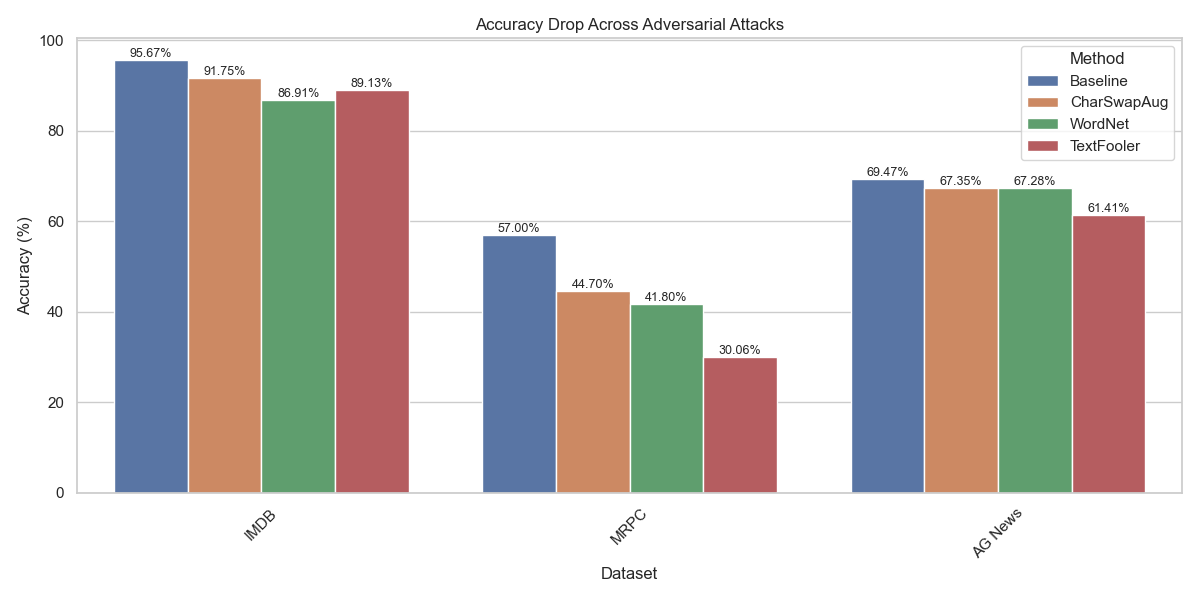
\includegraphics[width=0.9\linewidth]{figures/accuracy_chart_updated.png}
    \caption{Accuracy of Mistral-7B-Instruct under Baseline, CharSwapAug, WordNet, and TextFooler attacks across IMDB, MRPC, and AG News datasets.}
    \label{fig:accuracy}
\end{figure}

\textbf{SQuAD Results}:
\begin{itemize}
    \item F1 Score dropped from 31.11 (baseline) to 29.34 (CharSwapAug) and 28.36 (WordNet). Despite these drops, the model retained reasonable partial answer quality due to token overlap between adversarially perturbed inputs and gold answers.
    \item EM Score dropped from 1.00 (baseline) to 0.70 (CharSwapAug), but slightly increased to 1.20 (WordNet). This unexpected increase was likely due to coincidental synonym substitutions matching the gold answer by chance, rather than a real robustness gain.
\end{itemize}


\begin{figure}[htbp]
    \centering
    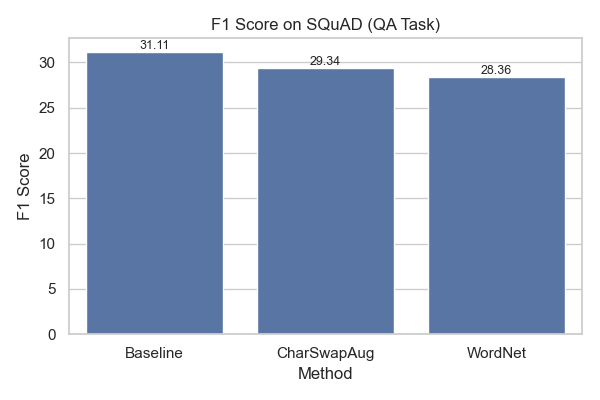
\includegraphics[width=0.65\linewidth]{figures/f1_chart_updated.png}
    \caption{F1 Scores of Mistral-7B-Instruct on SQuAD under Baseline, CharSwapAug, and WordNet attacks.}
    \label{fig:f1}
\end{figure}

\begin{figure}[htbp]
    \centering
    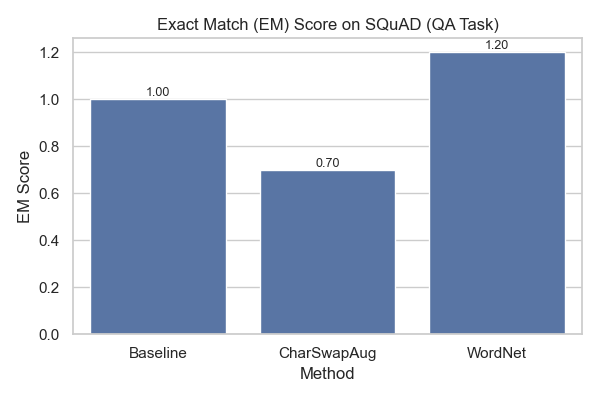
\includegraphics[width=0.65\linewidth]{figures/em_chart_updated.png}
    \caption{Exact Match (EM) Scores of Mistral-7B-Instruct on SQuAD under Baseline, CharSwapAug, and WordNet attacks.}
    \label{fig:em}
\end{figure}

Performance degradation was most severe on semantically sensitive tasks such as paraphrase detection (MRPC) and question answering (SQuAD), while sentiment classification (IMDB) and topic classification (AG News) comparatively demonstrated more robustness.

\subsection{Qualitative Results}

To better understand model failures, we manually analyzed 10 adversarial examples from the MRPC dataset.  
Key findings include:
\begin{itemize}
    \item When the model detected grammatical mistakes through swapping words (such as minor grammar or synonym changes) (e.g., ``buy'' $\rightarrow$ ``appear to buy''), the model often flagged grammatical inconsistencies but it failed to recognize the altered semantic meaning.
    \item Out of 10 adversarial MRPC examples tested, 5 were correctly classified and 5 were misclassified, indicating a 50\% accuracy rate under adversarial conditions.
    \item Semantic shifts based on WordNet synonym substitutions proved to be strong factors that led the model to produce incorrect predictions while maintaining proper grammar.
\end{itemize}


The research demonstrates Mistral-7B fails to preserve profound semantic consistency under surface-level adversarial perturbations.

\subsection{Analysis}

Task type proves to be a substantial determinant which influences how robust the system functions, according to the analytic findings:
\begin{itemize}
    \item Semantic tasks such as paraphrase detection (MRPC) are highly vulnerable to character- and word-level perturbations.
    \item Sentiment classification (IMDB) remains relatively resilient, because evaluating polarity is not dependent on precise word choices.
    \item Multi-class topic classification (AG News) experiences moderate, consistent degradation under attack.
    \item Question answering (SQuAD) shows some resilience in F1 score due to token overlap but remains susceptible under EM evaluation.
\end{itemize}

Interestingly, while both character-level (CharSwapAug) and word-level (WordNet) attacks caused measurable accuracy drops, TextFooler, a semantically preserving attack, had the greatest impact, especially on MRPC.

Confidence thresholding proved beneficial for preventing errors when under attack since it rejected predictions with low confidence rather than implementing incorrect predictions.

Thus, robustness is not solely a model training issue; it must be addressed holistically through better system design, including input handling and output management strategies.


\subsection{Summary}


In summary, the evaluation demonstrates that Mistral-7B-Instruct, while effective under clean conditions, remains vulnerable to adversarial attacks, especially in tasks requiring nuanced semantic understanding.  
Performance drops were most severe on paraphrase detection (MRPC) and question answering (SQuAD), while sentiment analysis and topic classification remained relatively stable.

Simple attacks such as CharSwapAug, WordNet synonym replacement, and TextFooler perturbations continue to pose a real risk to deployed LLMs.  
Our findings reinforce the need for task-specific evaluation, input sanitization pipelines, adversarial training, and confidence-based abstention mechanisms to build more robust and trustworthy LLM systems.


\section{Discussion}

This section outlines the logical next steps in response to our findings, including proposed defense mechanisms to enhance LLM robustness and suggestions for future research to strengthen adversarial resistance.

\subsection{Proposed Defense Mechanisms}

We outline three key defense mechanisms as natural and comprehensive defenses to the implemented attacks: \textbf{Adversarial Training}, \textbf{Input Preprocessing}, and \textbf{Embedding-Based Semantic Defense}.

\paragraph{Adversarial Training}
Adversarial training serves as a key defense for ensuring and increasing robustness against adversarial attacks. This is achieved by augmenting training data with perturbed samples. By integrating adversarial data generated from attacks such as \texttt{CharSwapAug} and \texttt{WordSwapWordNet}, the model’s training pipeline can be enhanced to improve generalization to adversarial inputs. Prior work by Jia and Liang \cite{jia2017adversarial} demonstrates the effectiveness of adversarial training in improving robustness, particularly for reading comprehension systems. We recommend incorporating paraphrase-based and synonym-substitution adversarial examples during fine-tuning to generate a more diverse and effective adversarial training set.

\paragraph{Input Preprocessing and Sanitization}
Input sanitization provides an alternative and complementary strategy, wherein adversarial noise is filtered prior to inference. This can involve the use of noise detection and removal algorithms, including text normalization techniques such as robust spell-checking, typo correction, and anomaly detection. These methods have been shown to improve model performance under attack \cite{omar2022robust}, particularly for character-level perturbations like those introduced by \texttt{CharSwapAug}. In the context of our work, the integration of preprocessing pipelines stands to significantly bolster LLM resilience.

\paragraph{Embedding-Based Semantic Defense}
Another promising approach for maintaining robustness involves preserving the semantic integrity of model embeddings in the presence of surface-level perturbations. As outlined by Huang and Chen \cite{huang2024semantic}, embedding-based semantic defense adjusts word embeddings using semantic associative fields, aligning them with the original context to suppress adversarial influence. This technique can be integrated into the model’s pipeline to protect against both word-level and character-level perturbations without altering the overall input semantics.

\subsection{Future Directions}

This section explores future research directions that build upon the findings of this project.

\paragraph{RL-Based Adaptive Attacks}
Reinforcement learning (RL)-based adaptive attack strategies have shown significant promise. RL agents can be trained to maximize attack success by dynamically adapting to model responses. Chen et al. \cite{chen2025worstcase} have demonstrated that such agents outperform static, rule-based approaches by discovering perturbation strategies in an online setting. Integration of RL-based perturbation generation presents a natural next step in adversarial evaluation.

\paragraph{Multimodal Robustness Testing}
Future research should also explore robustness beyond text-based inputs. Multimodal models such as LLaVA and GPT-4V, which process both textual and visual information, are increasingly deployed in real-world applications \cite{wsj2025securityrisks}. These models are susceptible to multimodal adversarial examples such as misleading images or mismatched captions. Building robust benchmarks and evaluation pipelines for such systems is essential to ensure reliability in these complex settings\cite{wsj2025securityrisks}.

\paragraph{Universal Robustness Enhancers}
Another area of interest lies in universal robustness strategies that aim to enhance model resilience by default. Recent work suggests the use of \textit{gradient-aligned preprocessing} to suppress adversarial noise without sacrificing semantic fidelity \cite{omar2022robust}. When combined with \textit{curriculum-based adversarial training}—wherein models are exposed to progressively difficult adversarial examples—this approach can continuously reinforce model robustness over time. Such strategies represent a long-term path toward inherently robust LLMs.

\bigskip
Ultimately, a combination of adversarial training, semantic defense techniques, multimodal evaluation, and dynamic adversarial agents can lead to a more trustworthy and secure deployment of LLMs in real-world settings.

\section{Conclusion}

Our work sought to test LLM robustness against a plethora of adversarial attacks, ultimately resulting in the implementation of attacks which caused meaningful degradation of LLM performance, with semantic tasks (MRPC) being most impacted. Specifically, character-level attacks and TextAttack augmentation implemented, WordNet attacks being evenly effective across the board, with proving to be TextFooler highly effective across all tasks/datasets. Subsequently, we presented tailored defense strategies for further reinforcing model robustness, and provided future directions, e.g., RL-based attacks, multimodal extensions, for consideration.


\section*{Author Contributions}

All authors contributed equally to the project. Below is a summary of individual roles:

\begin{itemize}
    \item \textbf{Anmol Devgun}: 
    \item \textbf{Anu Parbhakar}: Conducted the initial literature review on adversarial attack strategies, selected and implemented the target model for evaluation, and developed all baseline experiment scripts. Led the implementation of the TextFooler attack and corresponding experimental setup. Authored the Abstract, TextFooler subsection of the Approach, Implementation Design, Discussion, and Conclusion sections of the paper, as well as contributed to the presentation materials.
 
    \item \textbf{Youssef Ibrahim}: Responsible for analyzing the model’s performance degradation under adversarial attacks across datasets such as SQuAD, IMDB, MRPC, and AG News. Designed and implemented the accuracy, F1, and EM score visualizations comparing baseline and adversarial conditions (CharSwapAug, WordNet, TextFooler). Conducted in-depth performance analysis across datasets, identifying task-specific vulnerabilities and explaining real-world robustness implications. Briefly proposed defense strategies including adversarial training and semantic consistency checks. Authored the Evaluation section for this paper and the presentation.

    \item \textbf{Yunus Said}: Led the implementation of the CharSwapAugmenter and WordSwapWordNet adverserial attacks, including the corresponding experimental setup. Excuted the baseline, WordSwapWordNet and CharSwapAugmenter experiments for the SQuAD, IMDB and AG News datasets and collected the results. Wrote the Abstract section of the report besides the TextFooler subsection.
\end{itemize}


\bibliographystyle{IEEEtran}
\bibliography{references}

\end{document}
